%! TeX root = report.tex

\section{M2: Spec 2: Fold-Based Specification}

\SpecTwo{} addresses some of the limitations inherent in the straightforward
translation of \SpecOne{} from the Python executable specification.

\subsection{Translating Recursive \tlap{} Operators}

The primary goal of \SpecTwo{} is to maintain the semantic structure of
\SpecOne{} while eliminating recursion. In \SpecOne{}, (mutually) recursive
operators model key aspects of protocol behavior, such as the block tree and
block justification. Apalache does not natively support recursive
operators\footnote{\url{https://apalache-mc.org/docs/apalache/principles/recursive.html}},
thus it cannot be used immediately to model-check \SpecOne{}. While the
explicit-state \tlap{} model checker TLC supports recursive operators, it does
not scale to model-checking of this problem.

To resolve this, we reformulate \SpecOne{} into \SpecTwo{}, by substituting
(mutually) recursive constructs with bounded
\texttt{fold}~operations\footnote{In functional programming, \texttt{fold} is a
higher-order function that accepts a combining operation and an iterable data
structure, and applies the operation to each element of the data structure
to compute a single return value. \texttt{fold} is also known as
\texttt{reduce} in some languages.}, which enable the same iterative
computations to be performed in a non-recursive manner. We provide a set of
translation rules to convert recursive operators to bounded \texttt{fold}
operations, see Appendix~\ref{subsec:recrules}.

Let's reconsider the example in Figure~\ref{tla_adr}. In
Figure~\ref{fig:relationship-folds}, we present its equivalent that is using
folds. Following the rules in Appendix~\ref{subsec:recrules}, we have
constructed an accumulator \texttt{FindAncestor} that is passed to the fold
operator. Its body represents a single iteration of the recursive definition: it
first checks if its second parameter, indicating if an ancestor-descendant match
has already been found, is \texttt{TRUE} -- in this case, it simply propagates
the result \texttt{Pair(last\_block, TRUE)} to the next iteration (this is
equivalent to the base case of the recursive definition). If the match has not
been found, it checks if the current block is the genesis block or an orphaned
block, and returns \texttt{FALSE} if it is. Otherwise, it retrieves the parent
block of the current block, checks if it is the ancestor block, and passes
\texttt{Pair(parent, parent = ancestor)} to the next iteration. We pass this
accumulator to the fold operator, together with the initial value and the
structure to fold over (in this case, a generic sequence of length
\texttt{MAX\_SLOT}, which ensures that the fold is performed over all blocks in
the chain).


\begin{figure}
  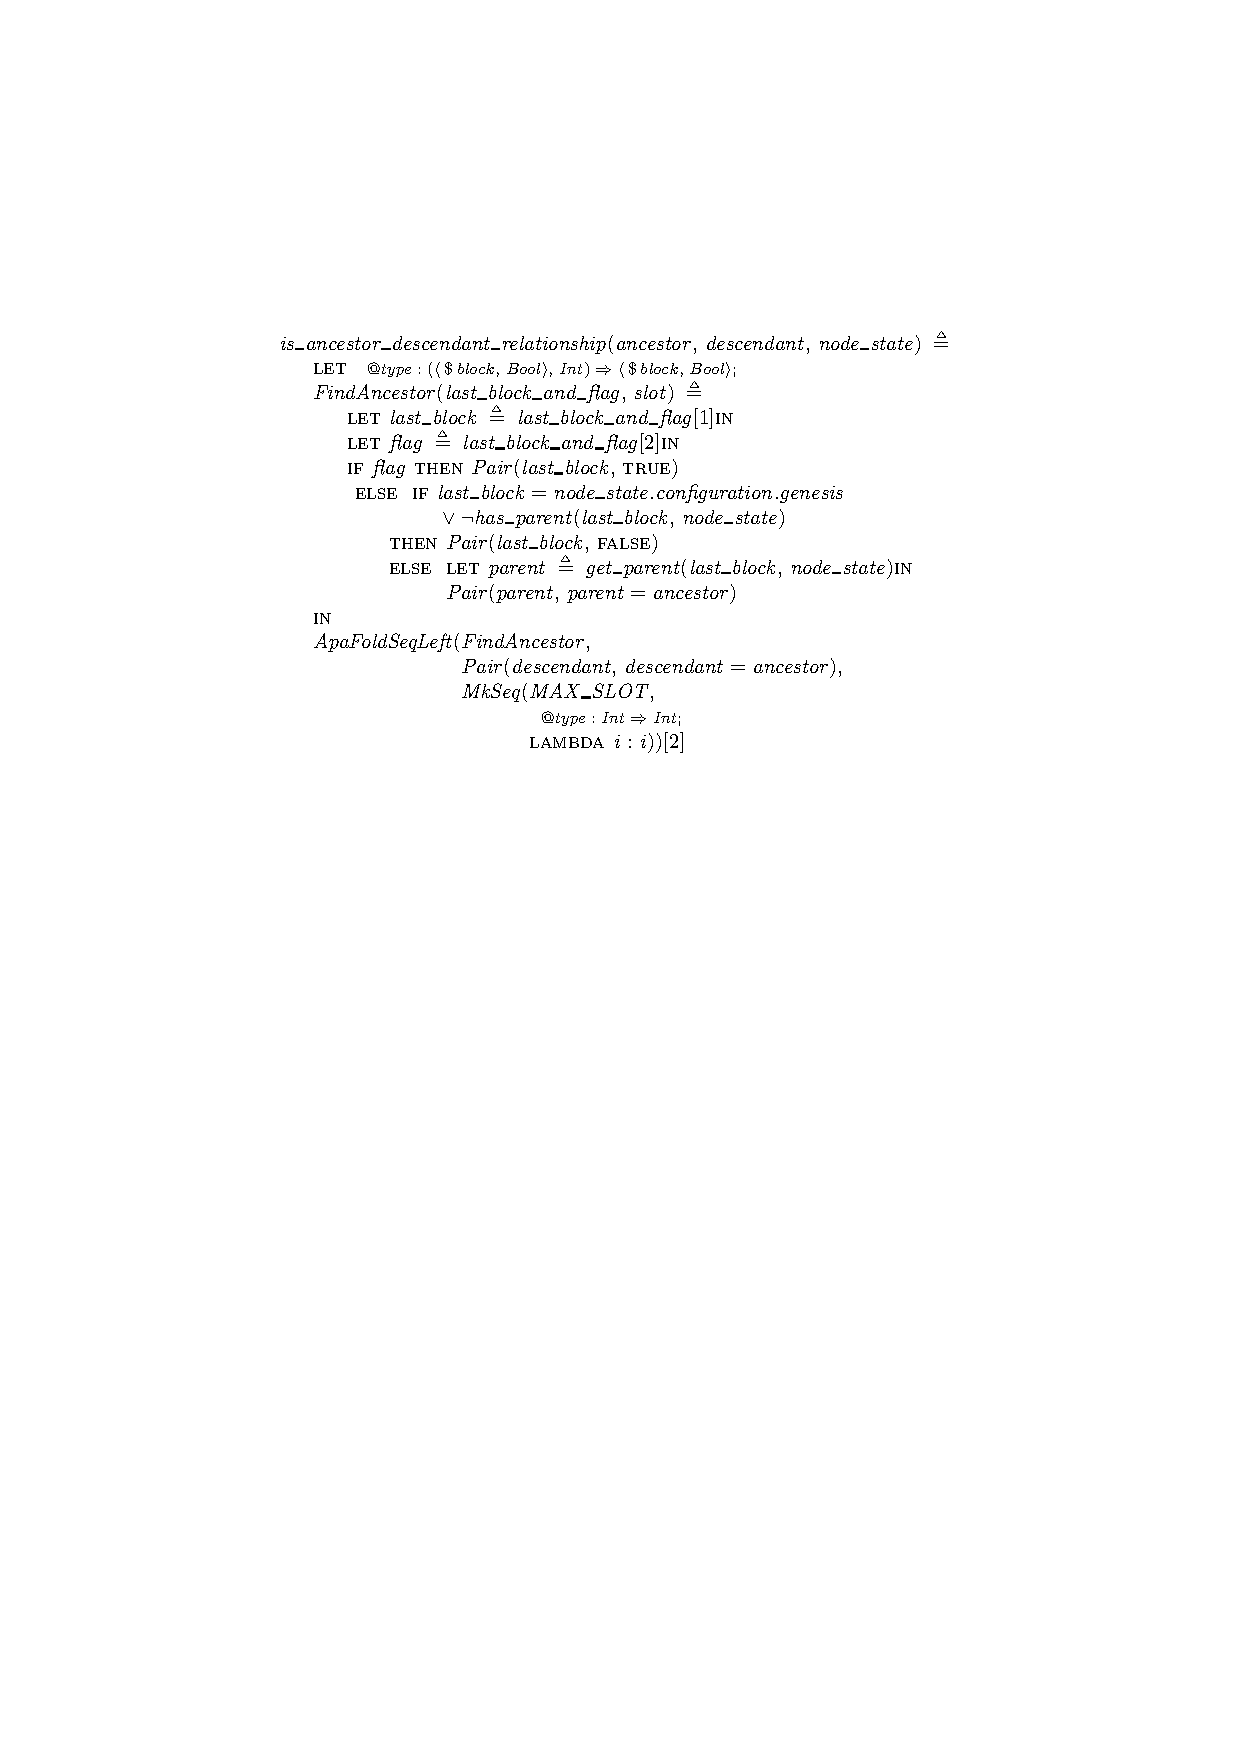
\includegraphics[width=\textwidth]{images/is_ancestor_descendant_relationship_folds.pdf}
  \caption{The recursive definition converted to bounded iteration with folds}%
  \label{fig:relationship-folds}
\end{figure}

\subsection{An Optimization: Flattening Nested Folds}

Initial model checking experiments with \SpecTwo{} revealed significant
challenges related to memory consumption, stemming from the high number of SMT
constraints emitted by Apalache for nested fold operations, which in turn mirror
the complexity of the original nested recursive structures from the Python
specification.

To address these issues, we introduce a manual optimization strategy that
involves flattening nested fold operations. This technique transforms nested
folds into a more manageable structure by employing additional \tlap{} state
variables, similar to memoization or prophecy variables.

For example, we introduce a new \tlap{} state variable
\texttt{PRECOMPUTED\_IS\_ANCESTOR\_DESCENDANT\_RELATIONSHIP} to store
memoized ancestor-descendant relationships and initialize it with the results
of the fold operation above, see Figure~\ref{fig:relationship-memo}.

\begin{figure}
  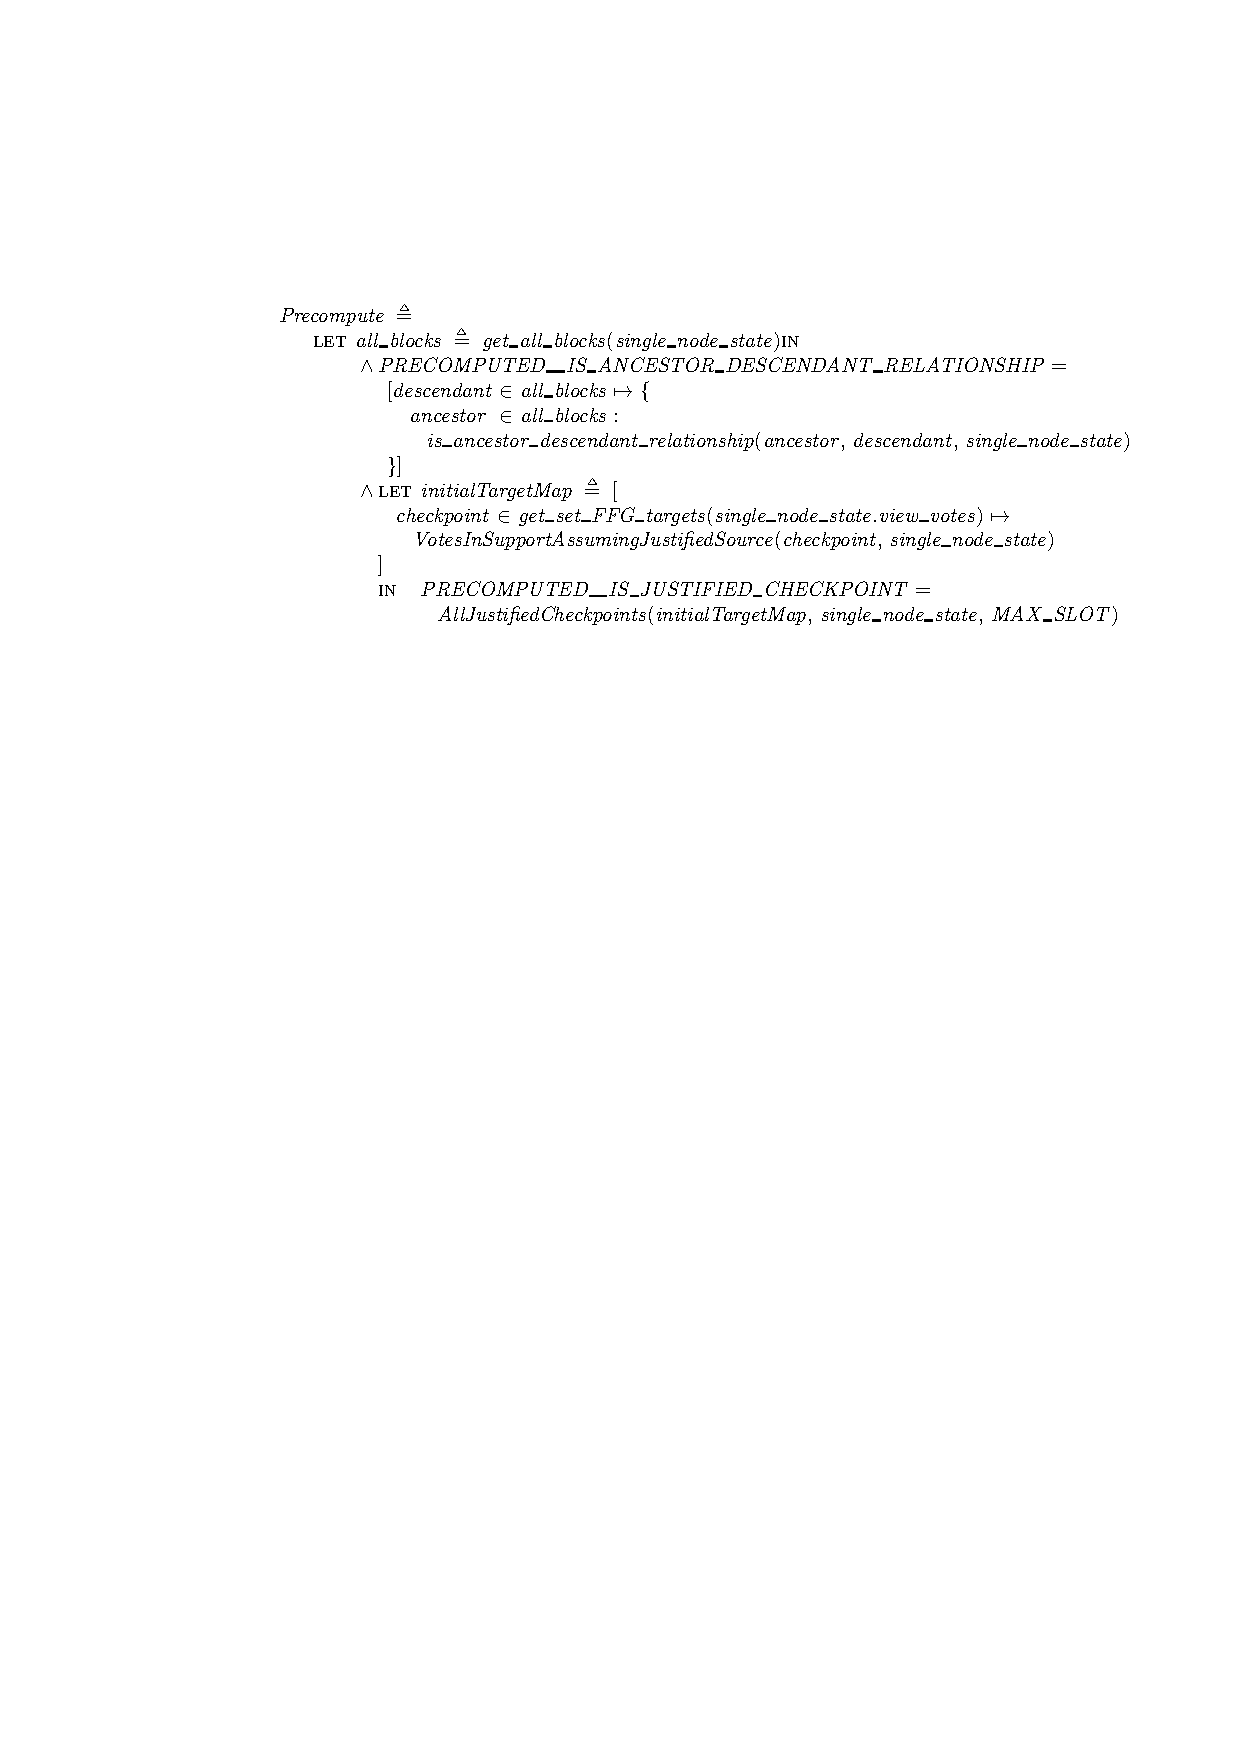
\includegraphics[width=\textwidth]{images/precompute.pdf}
  \caption{Memoizing the ancestor-descendant relationship}%
  \label{fig:relationship-memo}
\end{figure}

What does this give us? For instance, instead of re-evaluating the fold
operation each time we need to check if two blocks are in an
ancestor-descendant relationship, we can directly access the memoized result in
a much more efficient map lookup, as shown in
Figure~\ref{fig:conflicting-memo}.

\begin{figure}[h]
  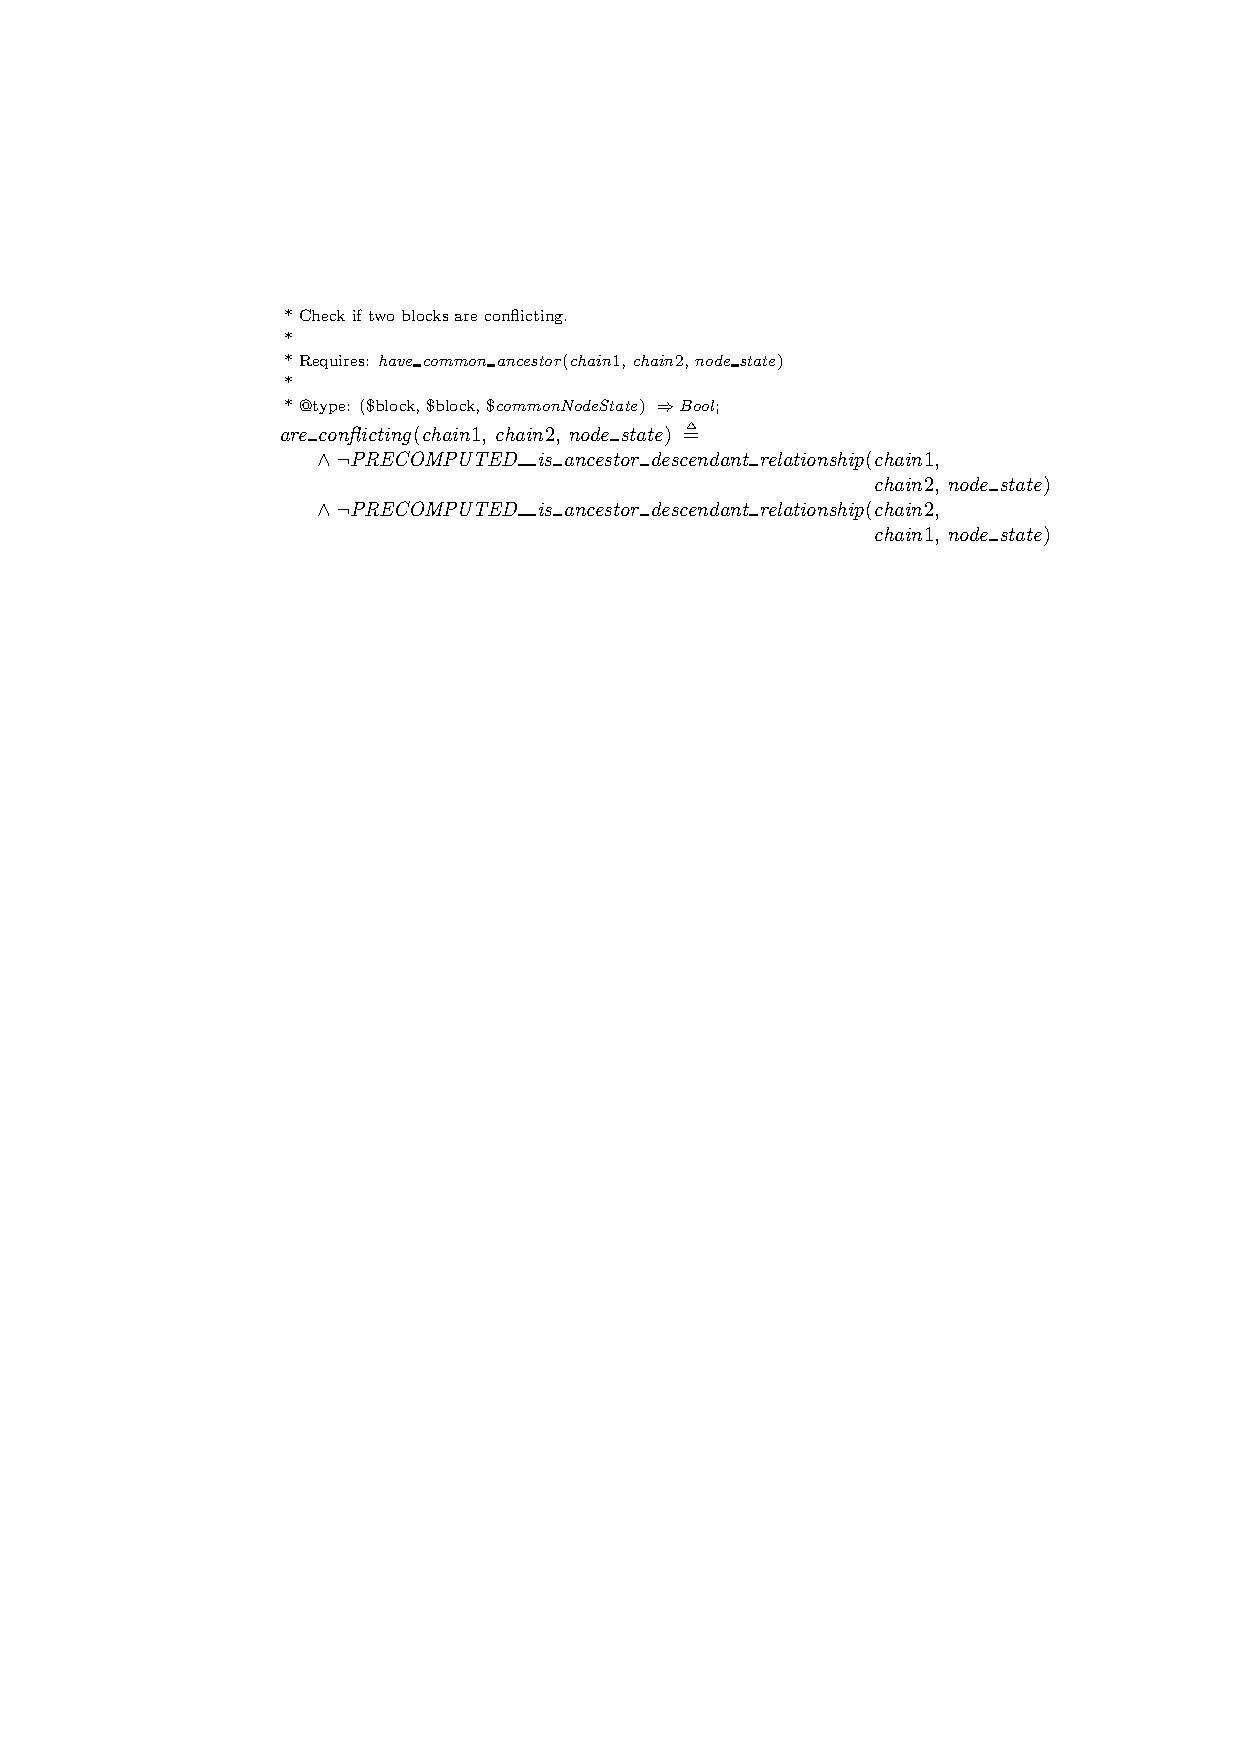
\includegraphics[width=\textwidth]{images/are_conflicting.pdf}
  \caption{The definition of conflicting blocks, using memoization}%
  \label{fig:conflicting-memo}
\end{figure}

To further improve our confidence in the correctness of this optimization, we
could produce a proof in TLAPS or run Apalache to show functional equivalence.

\subsection{Checking the Specification}

We can query the specification for reachable protocol states using Apalache.
For example, we can check if a nontrivial finalized checkpoint exists by writing an
invariant that we expect not to hold. If the invariant below is violated,
Apalache will produce an example of a finalized checkpoint as a counterexample,
see~Figure~\ref{fig:finalized-example}.

\begin{figure}[h]
  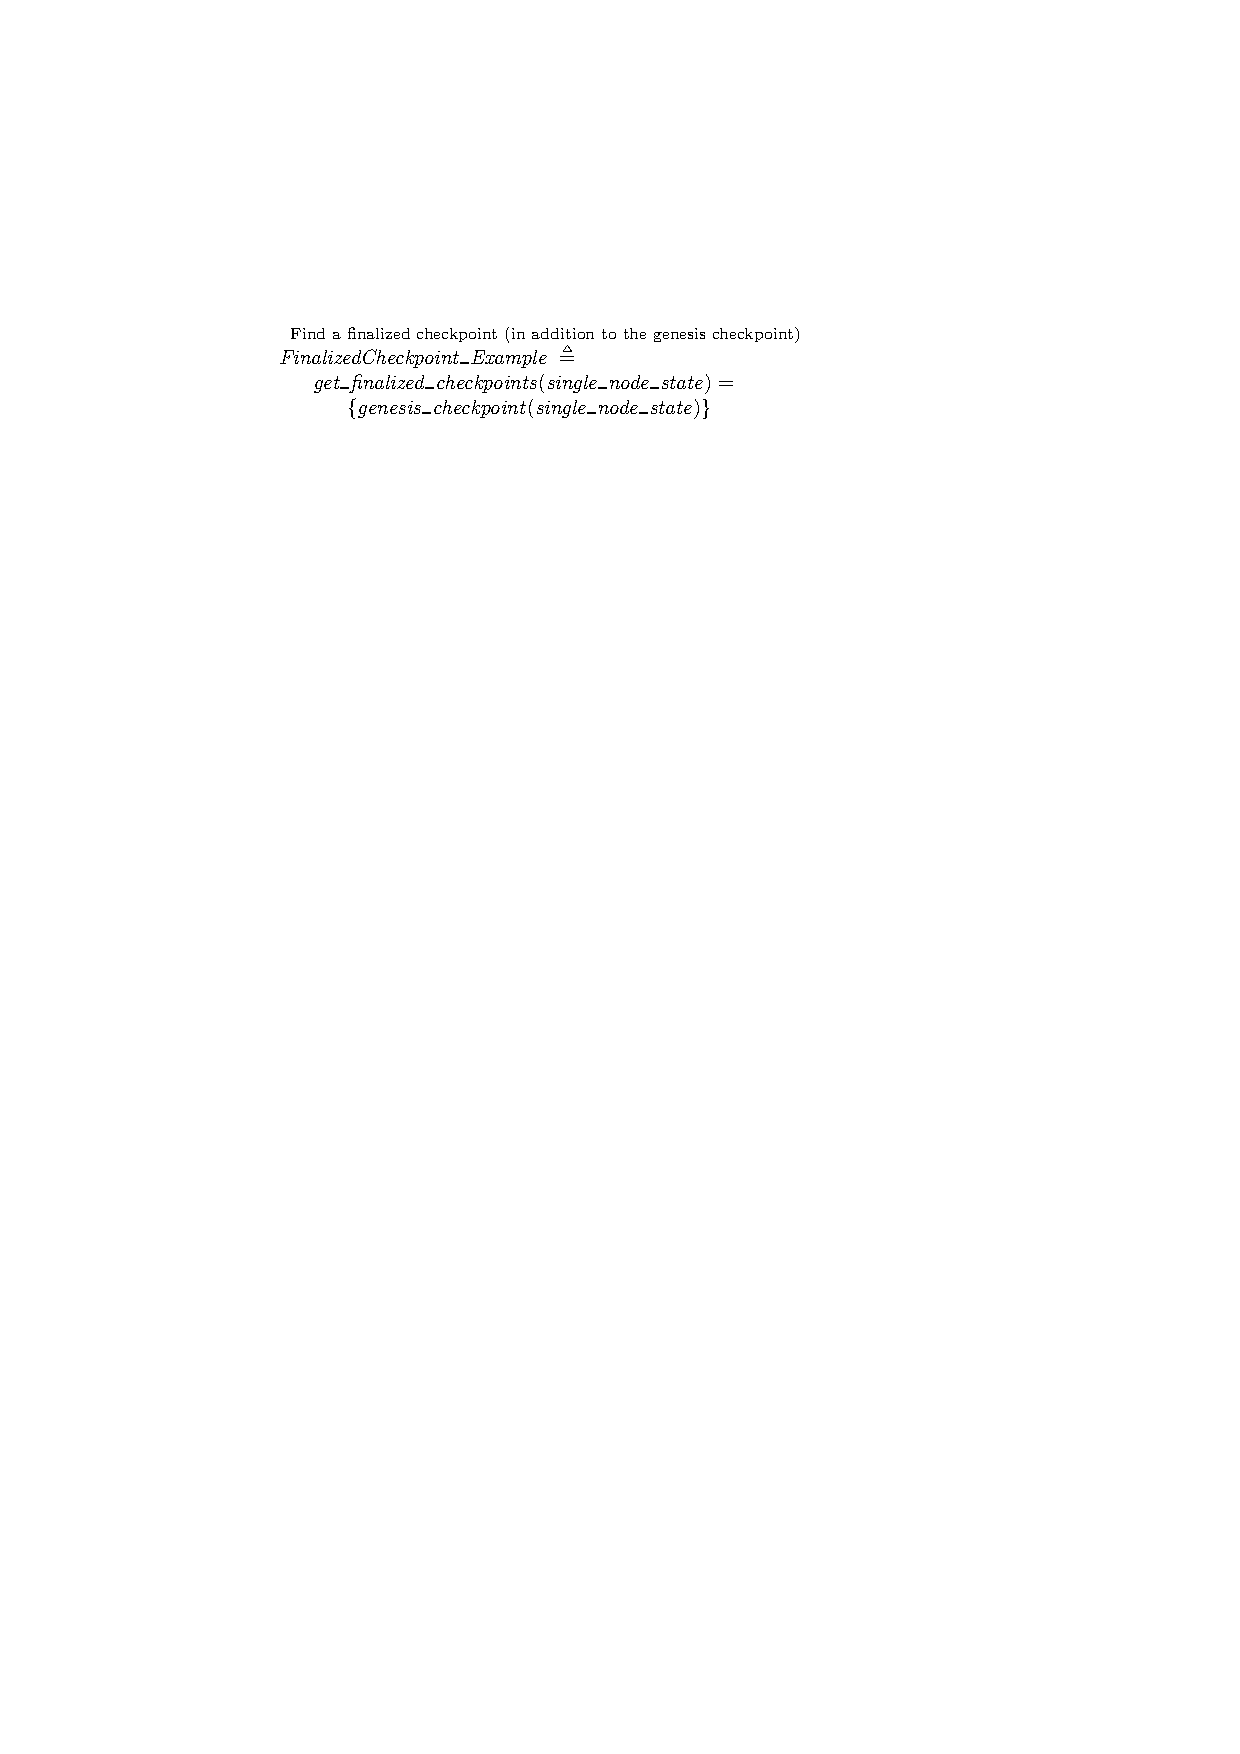
\includegraphics[width=\textwidth]{images/finalized-example.pdf}
  \caption{A false invariant for producing an example}%
  \label{fig:finalized-example}
\end{figure}

Obviously, we can also check \textit{AccountableSafety} by supplying it as an
invariant to Apalache, see~\ref{fig:accountable-safety}.

\begin{figure}[h]
  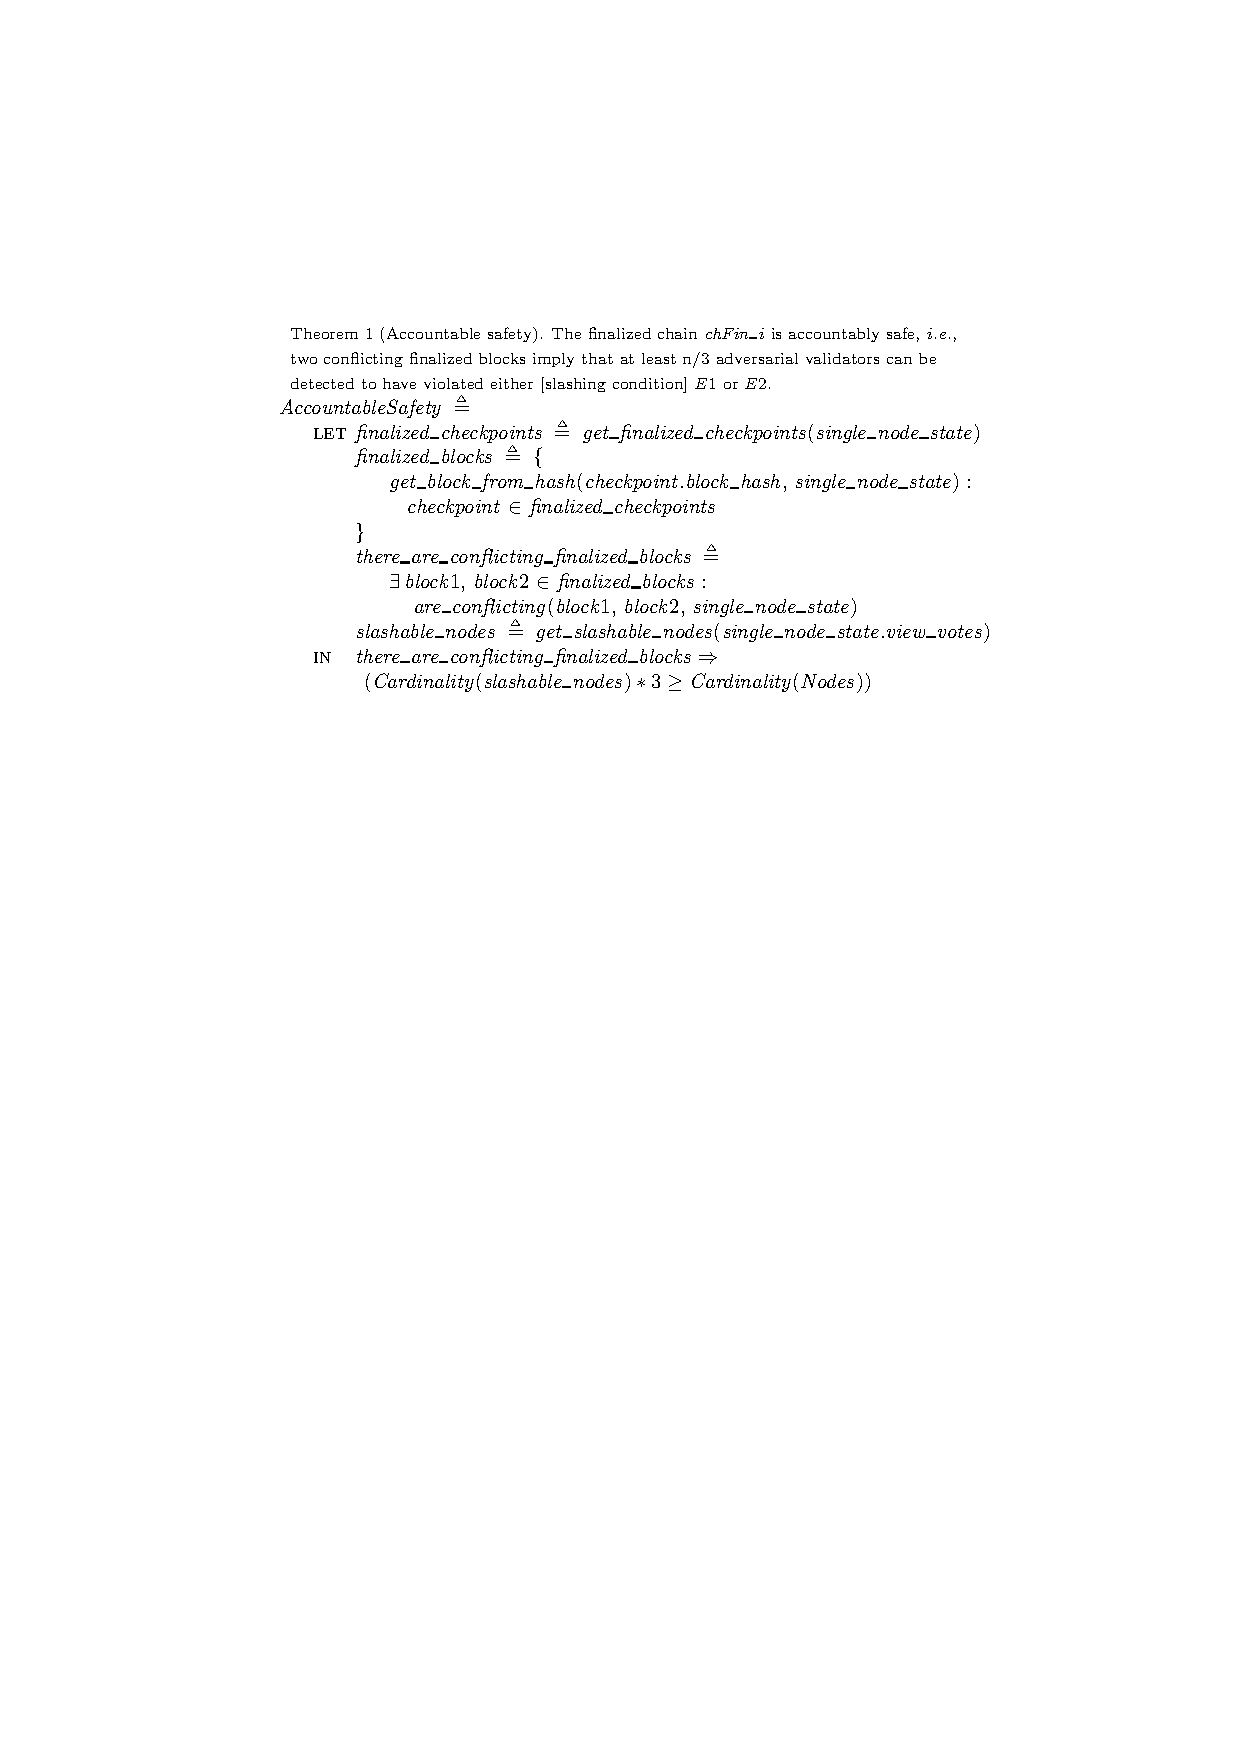
\includegraphics[width=\textwidth]{images/accountable-safety.pdf}
  \caption{A state invariant for accountable safety}%
  \label{fig:accountable-safety}
\end{figure}

Table~\ref{tab:spec2} shows the results of model checking \SpecTwo{} with
Apalache. We can see that generating examples of reachable protocol states and
verifying \textit{AccountableSafety} is infeasible due to the high computational
complexity of the specification.

\begin{table}
    \centering
    \begin{tabular}{ll}
        \tbh{Property} & \tbh{Time} \\ \toprule
        Example: conflicting blocks & timeout ($>40$h) \\
        Example: finalized \& conflicting blocks & timeout ($>40$h) \\
        AccountableSafety & timeout ($>40$h) \\ \bottomrule
    \end{tabular}
    \caption{Model checking \SpecTwo{} with Apalache.}\label{tab:spec2}
\end{table}

These results are not surprising -- the solver has to consider both reachability
properties for all possible block graphs, and all possible FFG voting scenarios
on top of these graphs. To further evaluate \SpecTwo{}, we fix the block graph
-- this way the solver only has to reason about voting. We encode three example
block graphs: a single, linear chain (\texttt{SingleChain}), a minimal forked
chain of three blocks (\texttt{ShortFork}), and a forest of disconnected chains
(\texttt{Forest}). Table~\ref{tab:spec2_fixed} shows the results of model
checking \SpecTwo{} for these fixed block graphs.

\begin{table}
    \centering
    \begin{tabular}{llr}
      \tbh{Property} & \tbh{Block graph} & \tbh{Time} \\ \toprule
      Example: conflicting blocks & \texttt{SingleChain} & 1 min 3 sec \\
      Example: conflicting blocks & \texttt{ShortFork} & 52 sec \\
      Example: conflicting blocks & \texttt{Forest} & 2 min 21 sec \\ \midrule
      Example: fin.\ \& confl.\ blocks & \texttt{SingleChain} & 1 min 5
      sec \\
      Example: fin.\ \& confl.\ blocks & \texttt{ShortFork} & 10 hours
      49 min 47 sec \\
      Example: fin.\ \& confl.\ blocks & \texttt{Forest} & timeout
      ($>40$h) \\ \midrule
      AccountableSafety & \texttt{SingleChain} & 1 min 13 sec \\
      AccountableSafety & \texttt{ShortFork} & timeout ($>40$h) \\
      AccountableSafety & \texttt{Forest} & timeout ($>40$h) \\ \bottomrule
    \end{tabular}
    \caption{Model checking \SpecTwo{} for fixed block
    graphs.}\label{tab:spec2_fixed}
\end{table}

We can see that the solver can handle the single chain block graph (where
\textit{AccountableSafety} trivially holds due to absence of conflicting
blocks), but struggles with the more complex scenarios even when given a fixed
block graph. This suggests that the complexity inherent in the specification is
due to the high combinatorial complexity of voting scenarios, rather than just
the block graph.
